\chapter{Einleitung}
\label{chap:einleitung}

Speedrunning bezeichnet die Praxis, Videospiele so schnell wie möglich abzuschließen. Was ursprünglich als Nischenbeschäftigung begann, hat sich zu einer globalen Wettbewerbskultur mit eigenen Events, Kommentatoren und einer kontinuierlich wachsenden Online-Community entwickelt. Die Plattform speedrun.com fungiert dabei als zentrale Infrastruktur: Sie sammelt, verifiziert und archiviert Weltrekordversuche aus tausenden von Spielen und stellt die historischen Daten über eine öffentliche API bereit~\cite{speedruncom_api}.

Aus datenwissenschaftlicher Perspektive bieten Speedrunning-Weltrekorde ein besonders geeignetes Untersuchungsobjekt. Alle Laufzeiten werden in Sekunden gemessen und von der Community verifiziert; der Beobachtungszeitraum reicht bei einigen Spielen bis in die 1990er~Jahre zurück. Die hierarchische Datenstruktur nach Genre und Kategorie ermöglicht systematische Gruppenvergleiche. Der Verlauf von Weltrekorden lässt sich als kollektiver Optimierungsprozess interpretieren: Eine dezentrale Community entdeckt schrittweise neue Routen, Bewegungstechniken und Programmfehler (sogenannte \emph{Glitches}), die kürzere Durchläufe ermöglichen.

\section*{Forschungsfragen}

Diese Ausarbeitung untersucht anhand eines selbst erhobenen Datensatzes aus 17~Spielen in sieben~Genres drei Forschungsfragen:

\begin{enumerate}
    \item \textbf{Zeitreduktion:} Wie stark hat sich die Bestzeit prozentual je Spielkategorie reduziert, und unterscheiden sich Genres systematisch in ihren Verbesserungsraten?
    \item \textbf{Sättigung:} Folgt die Verbesserungsrate einem erkennbaren mathematischen Muster, und gibt es einen statistisch nachweisbaren Sättigungspunkt?
    \item \textbf{Lebensdauer:} Wie lange hält ein Weltrekord im Mittel, und unterscheidet sich die Lebensdauer zwischen Genres und Jahrzehnten?
\end{enumerate}

Abbildung~\ref{fig:kaos} zeigt den KAOS-Baum,\footnote{KAOS: Konzepte, Annahmen, Operationen, Struktur --- ein Modell zur Strukturierung von Forschungsfragen.} der die Beziehungen zwischen den Forschungsfragen, dem Datensatz und dem Analyseziel darstellt.

\begin{figure}[htb]
  \centering
  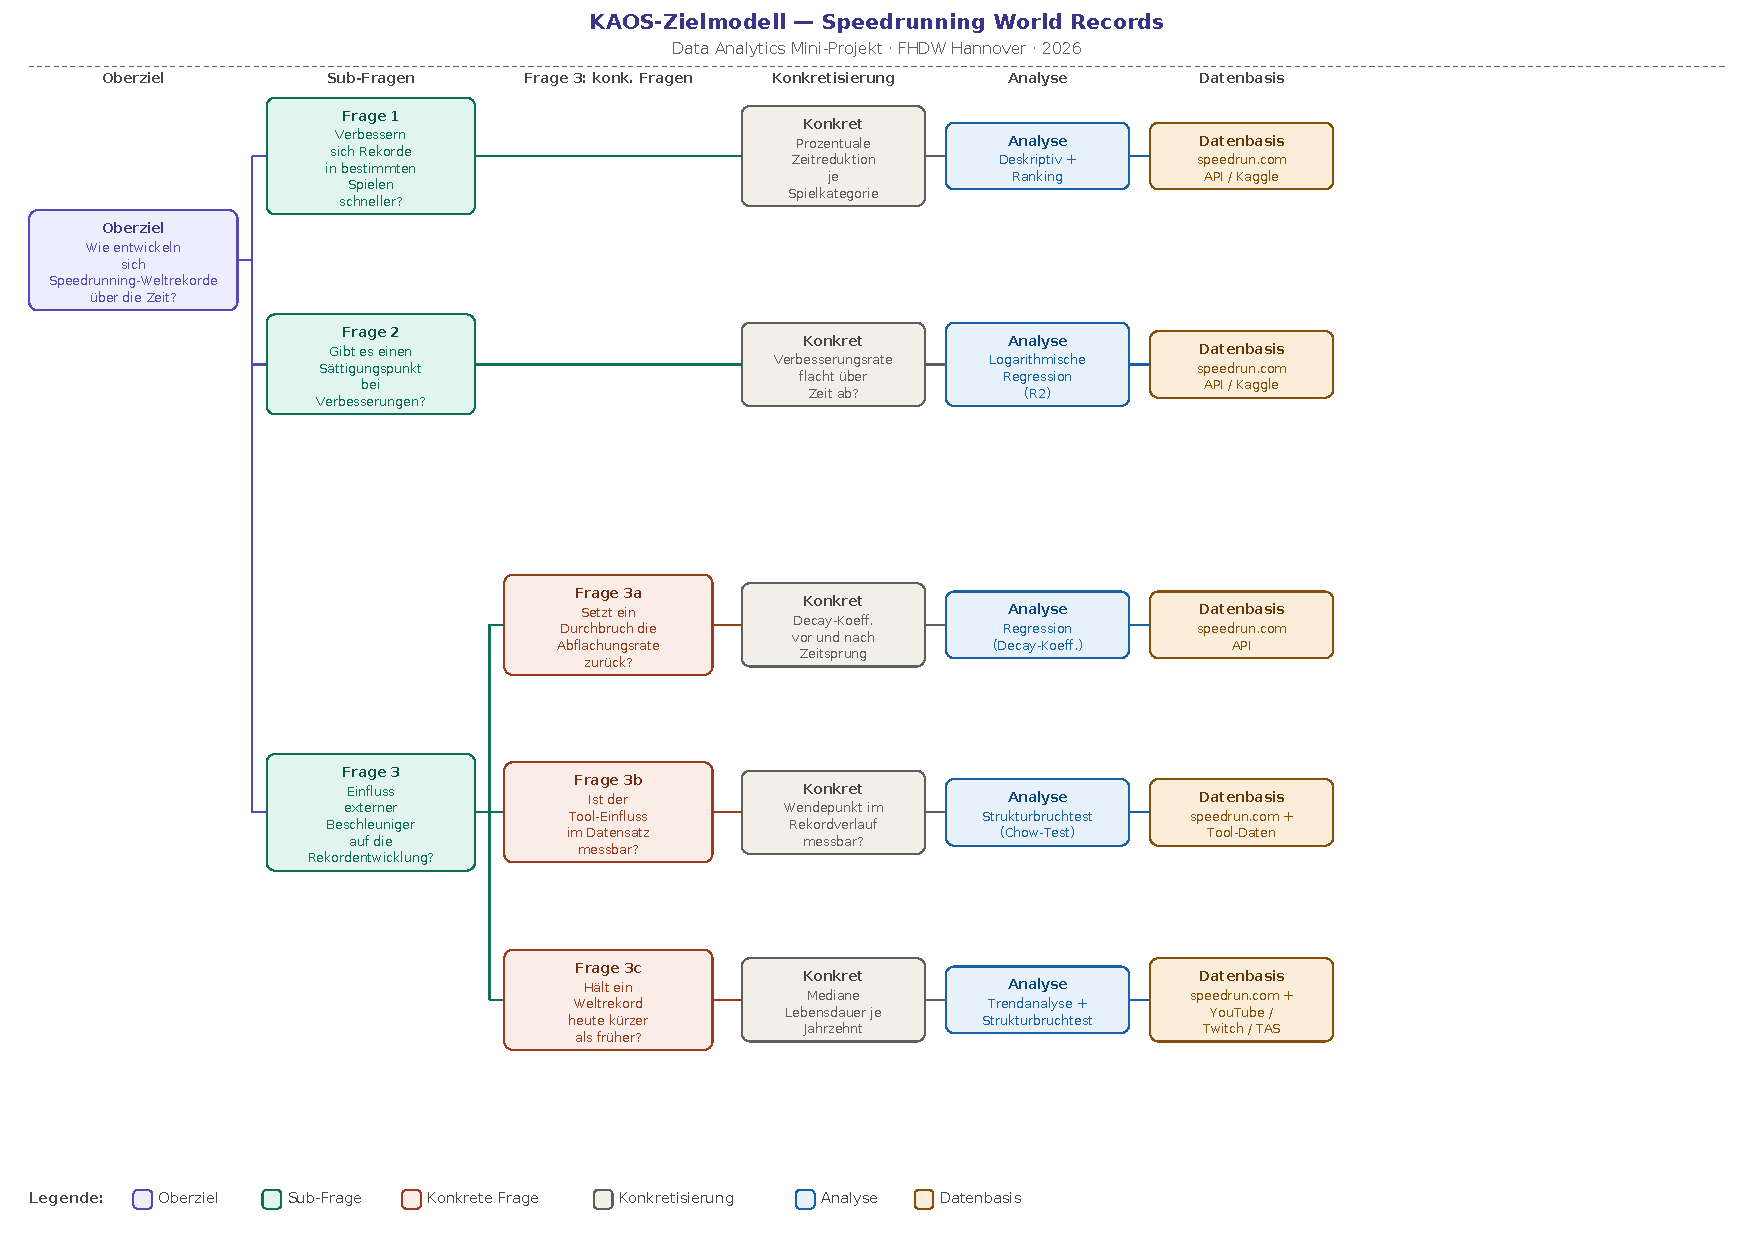
\includegraphics[width=0.55\textwidth]{contents/figures/kaos}
  \caption{KAOS-Baum der Speedrunning-Weltrekordanalyse}
  \label{fig:kaos}
\end{figure}

Die Ausarbeitung beschreibt zunächst Datenbasis und Methodik (Kap.~\ref{chap:methodik}), präsentiert die Ergebnisse zu allen drei Forschungsfragen (Kap.~\ref{chap:ergebnisse}), diskutiert Befunde und Limitationen (Kap.~\ref{chap:diskussion}) und schließt mit einem Fazit (Kap.~\ref{chap:fazit}).
